\chapter{Výskum a výsledky}\label{chap:results}
V tejto kapitole sa budeme venovať metódam a postupom vykonávania výskumu pre našu diplomovú prácu, vďaka ktorým sme sa dopracovali k finálnemu riešeniu našej práce. 

Ako prvé preskúmame few-shot object detection algoritmy a vyskúšame ako fungujú v praxi a ako ich môžme využiť v našej práci na učenie nových objektov a gest vďaka malému počtu anotovaných obrázkov. 

Preskúmal som dva prístupy:  Frustrantingly simple few shot object detection \cite{wang2020frustratingly}, Meta faster r-cnn: Towards accurate few-shot object detection with attentive feature alignment \cite{han2022meta}

Pri testovaní druhého spomínaného prístupu som zistil, že je príliš pamäťovo náročný a nebol som schopný ani po stiahnutí predtrénovaných modelov po prvých dvoch krokoch: meta-training, training base classes detection head, vykonať posledný pre mňa najôležitejší krok ktorý závisel na nových few-shot triedach (novel classes) fine-tuning. Moja grafická karta nemala dostatočnú pamäť 8GB a skúšal som to aj na virtual machine s grafickou kartou nvidia T4 16GB. 

Autori trénovali model na 4 20GB GPU. A ja som dostal nasledovný výstup aj po úprave trénovacích parametrov ako batch size, learning rate, tak aby stačilo čo najmenej pamäte: 

\begin{figure}[!hbt]
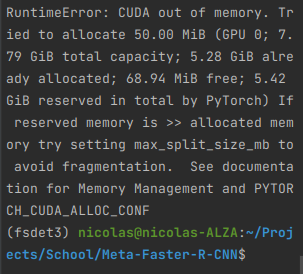
\includegraphics{images/no_memory.png}
\centering
\caption{Výstup pri fine-tuningu pomocou Meta Faster-RCNN}
\label{fig:image}
\end{figure}

Avšak Frustrantingly simple few-shot object detection prístup sa mi podarilo vyskúšať a otestovať, a po prispôsobení trénovacích parametrov k mojej obmedzenej pamäťovej kapacite som bol schopný spustiť všetky fázy tréningu. 

\section{Testovanie Frustrantingly simple few-shot object detection}

\subsubsection{Dataset:}
Pri few-shot object detection, potrebujeme mať dataset rozdelený na triedy ku ktorým máme veľké množstvo anotovaných dát(base classes), a na triedy ku ktorým máme malé množstvo anotovaných dát(novel classes).

Ako dataset som použil pascal voc, ako base classes som použil triedy:
aeroplane, bicycle, boat, bottle, car, cat, chair, diningtable, dog, horse, person, pottedplant, sheep,
train, tvmonitor.

Ako novel classes som použil triedy z pascal voc:
bird, bus, cow, motorbike, sofa a taktiež som pridal jednu vlastnu triedu apple(kde som anotoval 85
obrazkov pomocou labelImg), na trening(v druhej fáze pri finetuningu) bolo použitých len 5
obrázkov z každej triedy, ostatné boli použité na testovanie

Pre každú triedu som vytvoril 5-shot split, vybral som 5 obrázkov pre každú triedu pre fine-tuning.

\subsubsection{Tréning:}
Najprv som si stiahol predtrénovaný base model, ktorý bol trénovaný čisto iba na 15 base classes.
Následne som náhodne inicializoval váhy pre novel classes v poslednej vrstve modelu. A potom
som spustil finetuning poslednej vrstvy modelu.

Pri fine-tuningu som použil tieto paremetre:

\begin{figure}[!hbt]
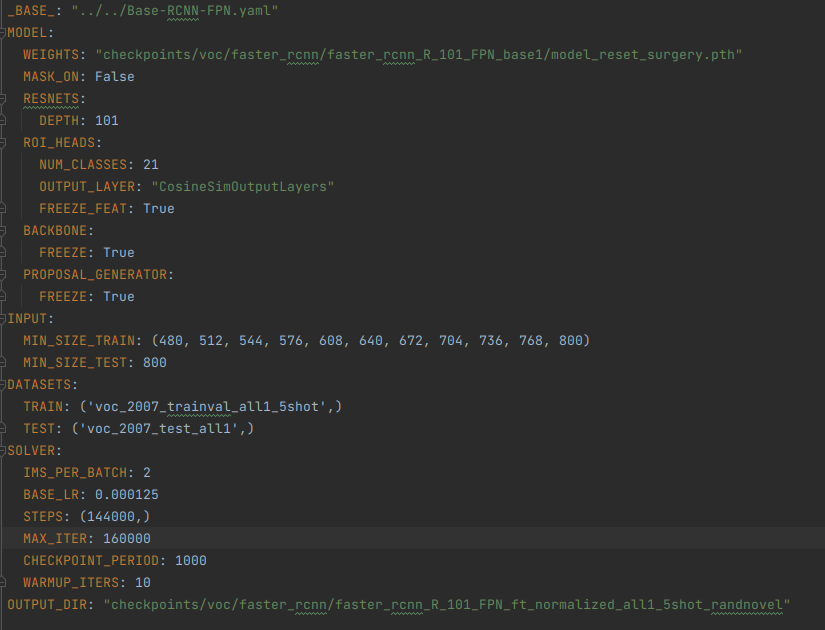
\includegraphics[width=\textwidth]{images/Training_parameters.png}
\caption{Tréningové parametre pri fine-tuningu}
\label{fig:image}
\end{figure}

\subsubsection{Vyhodnotenie:}

\begin{figure}[!hbt]
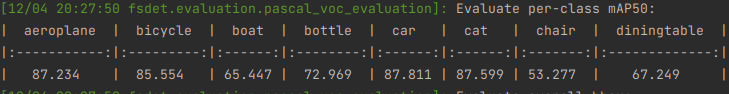
\includegraphics[width=\textwidth]{images/eval1.png}
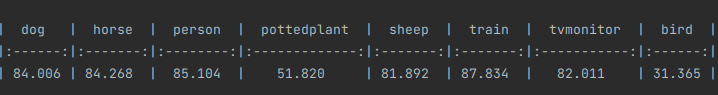
\includegraphics[width=\textwidth]{images/eval2.png}
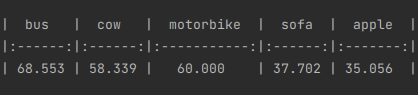
\includegraphics[width=\textwidth]{images/eval3.png}
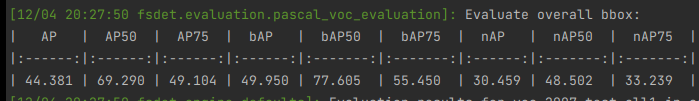
\includegraphics[width=\textwidth]{images/eval4.png}
\caption{Výsledky tréningu}
\label{fig:image}
\end{figure}


Ako vidíme hodnoty pre base classes nám ostali vysoké, a pri novel classes sa napriek tomu, že sme mali na tréning len 5 vzoriek a testovacia množina bola veľmi variabilná tak sme dostali mAP50 u každej novel class nad 30. 

Avšak myslel som si, že fine-tuning bude prebiehať veľmi rýchlo, keďže prebieha len na zopár obrázkoch z každej triedy a robot sa bude môcť učiť v real-time nové objekty, ale len samotný fine-tuning pri 5-shot trval na mojom GPU 5 hodín. Takže na učenie objektov v real-time sa to nebude dať použiť. Ale bude sa to dať použiť na učenie nových gest aj objektov, len pomocou zopár anotácií. 